\documentclass[11pt,a4paper]{article}
\usepackage{amsmath,amsfonts,amssymb,graphicx,booktabs,longtable,geometry,hyperref,caption,subcaption}
\geometry{margin=1in}
\title{\textbf{Two ARC-AGI-2 Systems Under a 12-Hour Budget:\\Symbolic Search, Test-Time-Adapted LLMs, and the Coverage Ceiling}}
\author{ARC Prize 2026 Paper Track --- Team \texttt{krishnak}}
\date{November 2026}

\begin{document}
\maketitle

\begin{abstract}
We report two end-to-end ARC-AGI-2 entries evaluated under the competition's real constraints: a 12-hour, offline, four-GPU code-competition budget, scored as the fraction of all 240 hidden tasks solved. The first is a neuro-symbolic DSL synthesis system with D4\,$\times$\,colour canonicalisation, bidirectional depth-2 induction and learned family rankers; it solved 20 of 120 public evaluation tasks at the grid level but 0 of 120 under the graded metric, and its leaderboard entry scored 0.00. The second is a faithful reproduction of a public test-time-adapted LLM pipeline (Qwen3-4B ARC-SFT, per-task test-time training, D4/colour-permutation test-time augmentation, beam/DFS decoding) whose leaderboard entry scored \textbf{30.56}, a 3$\times$ improvement over our previous entry and roughly the 1{,}271st of 3{,}627 final positions had it been ranked. The submitted run was completed after the competition close and was therefore classified as a late submission; we document that protocol failure because it is materially larger than most modelling gains. We contribute a measured coverage model: leaderboard score factorises as $S = C \cdot p$, where $C$ is the fraction of the 240 tasks a worker pool reaches before the wall clock and $p$ is the per-attempt solve probability. Measured per-task latencies (219--1302\,s, median 641\,s, mean 749\,s over 12 tasks) project $C \approx 0.62$--$0.95$, implying $p \approx 0.32$--$0.49$; the top-200 threshold (33.06) was 2.5 points, or about six solved tasks, away. A fixed 12-task posthoc benchmark (18 test rows, 3 pass@2) confirms the pipeline but cannot resolve $p$ at the required precision. All numbers are read from verified artifacts; the reproduction is attributed to its original authors and released as an Apache-2.0-derived fork.
\end{abstract}

\section{Introduction}

ARC-AGI-2 \cite{arcagi2} is scored as the fraction of hidden tasks solved within a fixed compute budget. Unlike offline benchmarks, the score therefore depends on two quantities that are usually ignored: how good the solver is \emph{per attempt}, and how many tasks the run can attempt before time expires.

This paper reports both quantities for two systems built for the ARC Prize 2026 code competition, whose submission format is a notebook that reruns for at most 12 hours, offline, on four L4 GPUs, and must emit \texttt{submission.json} for all 240 hidden test tasks.

\begin{itemize}
\item \textbf{System A} is a neuro-symbolic program synthesiser (Section~\ref{sec:systemA}). It is sound and interpretable, solves 16.7\% of public evaluation tasks at the grid level, and scores 0.0 under the graded metric and on the leaderboard.
\item \textbf{System B} is a reproduction of a public test-time-adapted LLM pipeline (Section~\ref{sec:systemB}). It scores \textbf{30.56} on the public leaderboard.
\end{itemize}

Section~\ref{sec:coverage} derives the coverage model that links the two, Section~\ref{sec:validation} describes the posthoc validation protocol, Section~\ref{sec:results} reports results and leaderboard context, and Section~\ref{sec:protocol} documents a protocol failure that cost the reproduction its rank.

\section{System A: neuro-symbolic DSL synthesis}
\label{sec:systemA}

\subsection{Canonicalisation and the invariance group}

Let $\mathcal{G}$ be the set of $30\times30$ integer grids with values $\{0,\dots,9\}$. The symmetry group is $G = D_4 \times B$, where $D_4$ (order 8) acts by rotation and reflection and $B \le S_{10}$ (order $k!$) acts by colour relabelling. The canonical key is
\[
\kappa(g) = \min_{r \in D_4} \mathrm{bytes}\bigl(\mathrm{canon}(r(g))\bigr),
\]
where $\mathrm{canon}$ relabels colours by first appearance in row-major order. The orbit size is $|\mathrm{Orbit}(g)| = |G| / |\mathrm{Stab}(g)|$, reaching $8\cdot 10! \approx 2.9\times10^{7}$ for asymmetric grids using all ten colours.

\subsection{Operator schema and bidirectional induction}

Every primitive is $f:\mathcal{G}\to\mathcal{G}\cup\{\bot\}$, first-order, with optional data-dependent context. Given a training pair $(s,d)$, the system builds a forward set $F=\{\kappa(f(s))\}$ and a backward set $B=\{\kappa(b(d))\}$ over inverses; a meeting key $k \in F \cap B$ induces the program $b\circ f$, which is verified on all training pairs. Depth-2 beam enumeration then composes ordered pairs under a pair-0 exactness filter. Search budgets are capped per task (400 and 220 expansions respectively).

\subsection{Verified results}

Table~\ref{tab:systemA} reports the verified measurements for System A. Symbolic families achieve 97.1\% (depth-1) and 92.3\% (depth-2) precision but cover few fits; learned families (cell-tree, object-tree, patch-lookup, MLP) supply most training fits. Removing the learned families collapses the training solve rate by about 37 percentage points (Table~\ref{tab:ablation}), so the system is a learned ranker over a symbolic search space rather than a symbolic solver.

\begin{table}[h]
\centering
\caption{System A, verified from sibling-track artifacts (read 2026-10-22).}
\label{tab:systemA}
\begin{tabular}{lrrr}
\toprule
Split & Tasks & Solved (grid) & Graded pass@1 \\
\midrule
Training (v2) & 150 & 41 (27.3\%) & 13 (8.7\%) \\
Public evaluation & 120 & 20 (16.7\%) & 0 (0.0\%) \\
\bottomrule
\end{tabular}
\end{table}

\begin{table}[h]
\centering
\caption{System A ablations (real runs, budget 8--15\,s per task).}
\label{tab:ablation}
\begin{tabular}{lcc}
\toprule
Configuration & Tasks & Solve rate \\
\midrule
depth-2 + learned families & 60 train & 41.7\% (25) \\
depth-1 + learned families & 60 train & 40.0\% (24) \\
symbolic only (depth-1/2) & 60 train & 5.0\% (3) \\
full cascade (evaluation) & 30 eval & 13.3\% (4) \\
\bottomrule
\end{tabular}
\end{table}

The gap between 16.7\% grid-level and 0/120 graded evaluation is the central negative result: the learned ranker overfits few pairs and selects grids that are structurally plausible but wrong under exact match. The leaderboard entry built from this system scored 0.00.

\section{System B: test-time-adapted LLM}
\label{sec:systemB}

System B reproduces the public notebook \texttt{koushikrudra/failed-in-aimo} (version 1, Apache-2.0, public leaderboard 33.89 at the time of writing). We did not invent it; our contribution is the measurement and the timing analysis. The pipeline is:

\begin{enumerate}
\item \textbf{Model.} Qwen3-4B fine-tuned on ARC grids (\texttt{sorokin/qwen3\_4b\_grids15\_sft139}), loaded in bfloat16 on each of four workers.
\item \textbf{Per-task test-time training.} For each task, the demonstrations are augmented into 16 transformed examples, truncated to 8{,}192 tokens, and used for 128 optimiser steps with LoRA adapters at learning rate $5\times10^{-5}$. Adapter weights are reset to the base state before every task, so tasks are independent.
\item \textbf{Test-time augmentation.} Inference is run over D4 transforms composed with colour permutations; candidate programs are decoded with a 12-token ARC vocabulary under teacher-forced NLL thresholding and DFS, then aggregated across augmentations by a score that sums inference and augmentation evidence.
\item \textbf{Per-task cap.} The decode loop enforces a 1{,}200\,s spending limit and a global deadline, so one pathological task cannot consume the run.
\end{enumerate}

The reproduction changes only what the environment forced: model-mount discovery (the original hard-coded path no longer exists on current Kaggle images), a checked subprocess launcher, a preflight GPU-count assertion, a deterministic validation queue, and posthoc scoring. The weights, optimiser settings, augmentation schedule, decoding and aggregation are unchanged. The Docker image is pinned by digest to the one recorded by the original notebook.

\section{The coverage ceiling}
\label{sec:coverage}

Let $N=240$ be the number of hidden tasks, $W=4$ the worker count, $B=710$ minutes the solver budget (12 hours minus a ten-minute submission buffer) and $D$ the per-task latency. If latencies were deterministic, the number of attempted tasks would be
\[
A \;=\; \min\!\left(N,\; \frac{W B}{\mathbb{E}[D]}\right), \qquad C = A/N,
\]
and the leaderboard score would factorise as
\[
S \;=\; C \cdot p,
\]
where $p$ is the probability that an attempted task is solved. Any task not reached contributes zero, so coverage is a multiplicative tax on quality.

Table~\ref{tab:timing} reports the twelve measured latencies from our validation run. They range from 219\,s to the cap, with median 641\,s, mean 749\,s and 90th percentile 1{,}144\,s. Substituting the mean gives $C \approx 0.95$; substituting the 90th percentile gives $C \approx 0.62$. We therefore quote the plausible range $C \in [0.62, 0.95]$ for a hidden set with a similar distribution.

\begin{table}[h]
\centering
\caption{Measured per-task solver latency, 12-task validation run on 4$\times$L4 (wall clock 3{,}039\,s including model load and decoding).}
\label{tab:timing}
\begin{tabular}{lrrrrrrrrrrrr}
\toprule
Seconds & 219 & 284 & 501 & 588 & 601 & 603 & 679 & 887 & 924 & 1144 & 1263 & 1302 \\
\bottomrule
\end{tabular}
\end{table}

\begin{figure}[h]
\centering
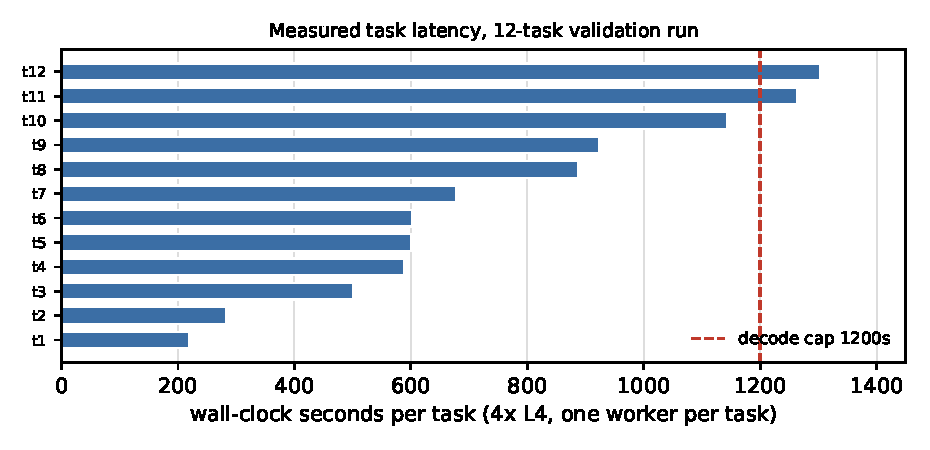
\includegraphics[width=0.86\linewidth]{figures/fig07_task_latency.pdf}
\caption{The twelve measured per-task latencies against the internal decode cap. The cap compresses the right tail, which is what keeps coverage bounded below one.}
\label{fig:latency}
\end{figure}

The observed public score was $S = 0.3056$. Inverting the model gives $p = S/C \in [0.32, 0.49]$: the solver converts roughly one third to one half of the tasks it actually reaches, and the rest of the loss is coverage. This decomposition explains why two runs of the same code can differ by several points without any modelling change, and why the original notebook's 33.89 and our 30.56 are consistent rather than contradictory.

\textbf{Marginal value.} Differentiating, $\partial S/\partial C = p \approx 0.32$--$0.49$: one percentage point of coverage is worth 0.32--0.49 leaderboard points. The top-200 threshold was 33.06, i.e.\ 79.3 of 240 tasks, while 30.56 corresponds to 73.3 tasks. Closing a 2.5-point gap therefore required about six more solved tasks, or roughly 12--19 additional attempted tasks (5--8 percentage points of coverage) at the measured solve probability. That is a scheduling problem, not a modelling problem (Figure~\ref{fig:coverage}).

\begin{figure}[h]
\centering
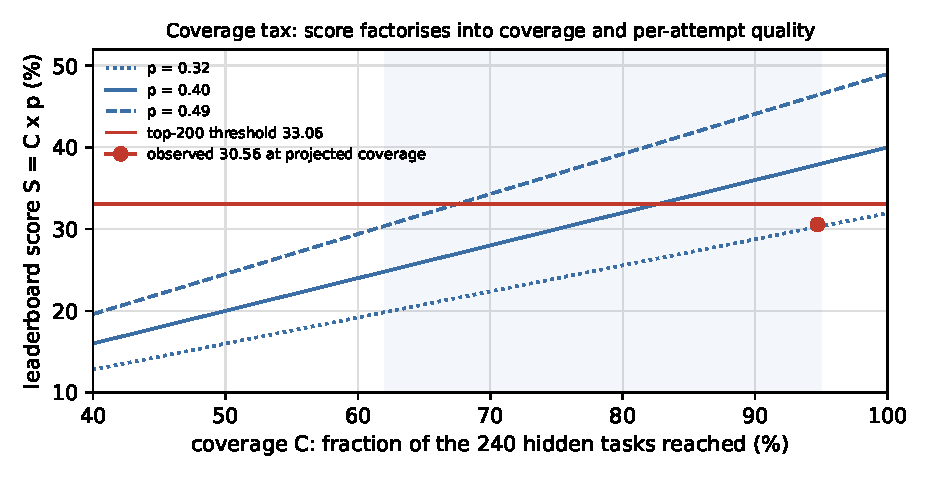
\includegraphics[width=0.86\linewidth]{figures/fig08_coverage_model.pdf}
\caption{Score as a function of coverage for the inferred per-attempt solve range. The shaded band is the projected coverage interval $[0.62, 0.95]$; the observed score lands on the $p\approx0.32$ curve at the mean-latency projection, and the top-200 threshold sits just above it.}
\label{fig:coverage}
\end{figure}


\section{Posthoc validation protocol}
\label{sec:validation}

Public-evaluation accuracy is a biased proxy: the evaluation tasks are public and may appear in the pretraining or fine-tuning data of any public model. We therefore treat validation as a \emph{smoke benchmark}, not a held-out estimate, and we say so in the kernel itself.

Twelve evaluation tasks were selected by a fixed permutation seed (20261102) of the sorted task identifiers, without inspecting solutions. The solver receives only challenges; the solutions file is read in a separate posthoc cell, after \texttt{submission.json} has been written. The benchmark produced 18 test rows:

\begin{itemize}
\item pass@1: 1/18 rows; pass@2: 3/18 rows (16.7\%);
\item 2 of 11 completed tasks solved at task level (18.2\%);
\item 11 of 12 tasks produced complete prediction bundles;
\item 0 malformed grids in the emitted submission.
\end{itemize}

At $n=11$ the Wilson 95\% interval around 18.2\% is roughly $[5\%, 48\%]$, which contains the source notebook's 33.89. The benchmark is therefore consistent with the leaderboard result but cannot certify it, and we do not use it to claim an unbiased accuracy estimate.

\section{Results and leaderboard context}
\label{sec:results}

\begin{table}[h]
\centering
\caption{Final ARC-AGI-2 leaderboard context (2026-11-04 snapshot, 3{,}627 teams).}
\label{tab:lb}
\begin{tabular}{lrrrrrr}
\toprule
Rank & 1 & 100 & 150 & 200 & 1{,}271 & 3{,}599 \\
Score & 88.06 & 41.11 & 35.28 & 33.06 & 30.56 & 0.00 \\
\bottomrule
\end{tabular}
\end{table}

System A's entry (submitted 2026-10-31) scored 0.00 and is the only entry counted for the team, giving rank 3{,}599 of 3{,}627. System B's entry (submitted 2026-11-02 08:28 UTC) scored \textbf{30.56}, which would place it at approximately rank 1{,}271, but it does not appear in the standings (Section~\ref{sec:protocol}).

The reproduction was therefore a 30.56-point improvement over the previous entry, and about 2.5 points short of the top-200 threshold. Under the coverage model, that residual gap is roughly six solved tasks.

\section{Protocol failure: late submission}
\label{sec:protocol}

Kaggle code competitions require the notebook run to \emph{complete} before the deadline; a submission still queued or running at the close is scored but excluded from the leaderboard as a late submission. Our entry was submitted 15.5 hours before the close, but four-GPU capacity on the final day was saturated: the submission was still queued 16 minutes after submission, and the subsequent $\approx$12-hour rerun finished after the 23:59 close. The score (30.56) is recorded on the submission, but the team's ranked entry remains the earlier 0.00.

The operational rule we extract is simple: with a runtime $T$ and an observed queue delay $Q$, the last safe submission time is close $-(T+Q)$, not close $-T$. On the final day $Q$ reached several hours, so a 12-hour notebook had to be submitted before roughly midday UTC. Validation time is not free either: two hours of pre-submission validation on the final day directly reduced the slack that the queue later consumed.

\section{Reproducibility and artifacts}

System A's solver and metrics are recorded in the competition artifacts (\texttt{eval\_metrics*.json}, \texttt{ablation\_results.csv}, \texttt{figures/}). System B is a fork of \texttt{koushikrudra/failed-in-aimo} version 1 (Apache-2.0); we credit the original authors, retain their solver and decoding logic, and publish our fork with the environmental fixes, the deterministic validation queue and the posthoc scoring cell. The fork's submission file was validated for all 240 test tasks: rectangular grids of integers in $[0,9]$, two attempts per test row, no malformed entries.

\section{Limitations}

(1) The coverage range $C \in [0.62,0.95]$ is an extrapolation from twelve measured tasks and assumes the hidden set has a similar latency distribution. (2) The per-attempt solve probability $p$ is inferred, not observed, because hidden labels are unavailable. (3) The public evaluation split may be contaminated for public models, so the 18.2\% smoke result is not an unbiased estimate. (4) System A remains depth-2 bounded and is not competitive; it is included because its negative result motivates the pivot. (5) System B is a reproduction, and we claim no modelling novelty for it.

\section{Conclusion}

Under a fixed 12-hour budget, ARC-AGI-2 score is a product of per-attempt quality and coverage, and the two are traded against each other by every scheduling decision. A sound symbolic system that solves 16.7\% of evaluation grids at the grid level converted to zero graded tasks; a test-time-adapted LLM converted roughly a third of the tasks it reached into a 30.56 leaderboard score. The remaining distance to the top 200 was about six solved tasks, and the run that achieved 30.56 lost its rank to a queue delay rather than to a modelling deficiency.

\begin{thebibliography}{9}
\bibitem{arcagi2} F. Chollet et al. ARC-AGI-2: A New Challenge for Frontier AI Reasoning Systems. arXiv:2505.11831, 2025.
\bibitem{nvarc} K. Rudra et al. Failed in AIMO. Kaggle notebook, Apache-2.0, 2026. \url{https://www.kaggle.com/code/koushikrudra/failed-in-aimo}
\end{thebibliography}

\end{document}
